\section{Oscillations and Waves}
As you have probably noticed, oscillations and waves play a major role in acoustics (and in many other areas of physics). To gain a better understanding, we will now examine the mathematical foundations and physical concepts in more detail.





\paragraph{General Form of Harmonic Oscillations}

\begin{figure}[!ht]
\begin{center}
    \begin{minipage}{0.52\textwidth}
        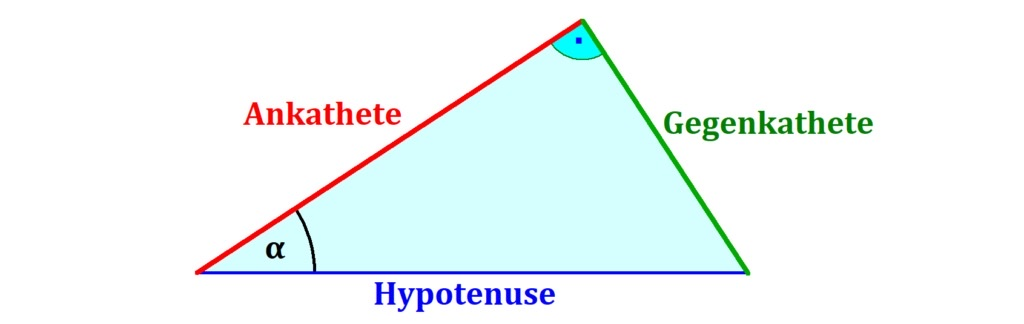
\includegraphics[width=\textwidth]{Bilder/rechtwinkliges Dreieck.jpeg}
        \caption{\footnotesize right-angled triangle}
        \label{img:rechtwinkliges_Dreieck}
    \end{minipage}
    \hfill
    \begin{minipage}{0.38\textwidth}
        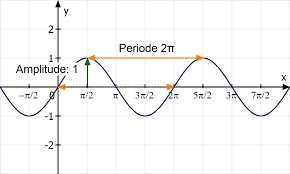
\includegraphics[width=\textwidth]{Bilder/Sinusfunktion.jpeg}
        \caption{\footnotesize Sine function}
        \label{img:sinusfunktion}
    \end{minipage}
\end{center}
\end{figure} 


A general harmonic oscillation can be written as:
\begin{equation}
     f(x)= a \cdot sin(b \cdot x+c)+d
\end{equation}

There are four parameters affecting the periodic function as described in the following :
\begin{itemize}
    \item $a$: amplitude (vertical stretching/compression)
    \item $b$: affects the period, with $b = \frac{2\pi}{T}$
    \item $c$: phase shift (horizontal shift)
    \item $d$: vertical shift
\end{itemize}

\paragraph{Cosine Function}
The cosine function is simply a phase-shifted sine function:
\begin{equation}
    \cos(x) = \sin\left(x + \frac{\pi}{2}\right)
\end{equation}

Thus, cosine functions can also describe harmonic oscillations:
\begin{equation}
    g(x) = a \cos(bx + c) + d
\end{equation}


\subsection{Mechanical Waves}
A particle which is capable of oscillating/vibrating is called oscillator. 
When several oscillators are coupled and set into motion, the oscillation propagates through space. We again consider harmonic waves, which can be described using sine and cosine functions. A wave is therefore a spatial and temporal periodic change of physical quantities.
If you observe the space at intervals of one period
T, it appears unchanged each time. If all coupled oscillators reach their maximum amplitude at the same time, we say that the oscillators are 'in phase'.
In the case of water waves, the individual oscillators are the water molecules that oscillate back and forth.
They are coupled to one another via hydrogen bonds. The following quantities are suitable for describing
mechanical, harmonic waves:
\begin{itemize}
    \item \textbf{Period $T$}: time for one complete oscillation
    \item \textbf{Frequency $f$}: number of oscillations per unit time, $f = \frac{1}{T}$
    \item \textbf{Wavelength $\lambda$}: shortest distance between two points oscillating in phase -- this is the distance from one wave crest to the next (or from one trough to the next), as can be seen directly in a position-displacement diagram.
    \item \textbf{Wave speed $c$}: speed at which the wave propagates
\end{itemize}
To describe and visualize waves physically, several types of diagrams are used. If we want to describe the state of space at a specific time $t_0$, a position-deviation diagram is suitable. In this diagram, you can see the deviation of different oscillators at a given time. On the x-axis, you find the distance of the oscillators from a reference point $x_0$, and on the y-axis their displacement can be seen. This allows you to determine the oscillators' distances from their equilibrium position at a certain time  $t_0$.   The left diagram in Figure \ref{img: harmonische Welle} shows such a position-displacement diagram. \\
If you want to describe the motion of an oscillator located at position $x_0$, we use a time-displacement diagram (see the right diagram in Figure \ref{img: harmonische Welle}). \footnote{https://www2.physki.de/PhysKi/images/thumb/7/76/Waveharm2.png/400px-Waveharm2.png}
\begin{figure}[!ht]
\begin{center}
    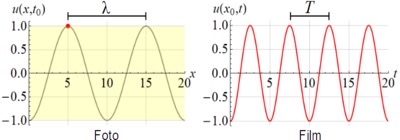
\includegraphics[height=4cm]{Bilder/Wellen.jpeg}
    \caption{\footnotesize harmonic wave}
    \label{img: harmonische Welle}
\end{center}
\end{figure}
\\
If you want to represent the temporal evolution of waves in space, position-displacement diagrams at different points in time are suitable. \footnote{https://www.leifiphysik.de/mechanik/mechanische-wellen/aufgabe/harmonische-wellen}
\begin{figure}[!ht]
\begin{center}
    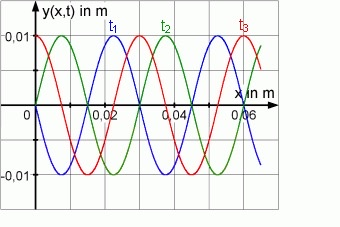
\includegraphics[height=4cm]{Bilder/fortschreitende Welle.jpeg}
    \caption{\footnotesize propagating harmonic wave}
    \label{img: fortschreitende Welle}
\end{center}
\end{figure}
\\

\paragraph{Relationship Between Wave Quantities}
The following relationship holds between the different wave quantities:
\begin{equation}
    c=\frac{\lambda}{T} = \lambda \cdot f
\end{equation}
This formula can be understood intuitively: within one second, $f$ complete waves pass a given point. Each wave has length $\lambda$. Therefore, the wave travels a total distance of $f \cdot \lambda$ per second -- and that is exactly the wave speed $c$.

\subsubsection{Different Types of Waves}
In order to describe a wave and its propagation through space even more accurately, we distinguish between two fundamental types of waves:
\begin{itemize}
    \item \textbf{Transverse waves}: the oscillators move \textbf{perpendicular} to the direction in which the wave travels. \\
    \textit{Example:} If you shake one end of a rope up and down, a wave travels along the rope horizontally while the rope itself moves vertically. Water waves behave similarly.
    \item \textbf{Longitudinal waves}: the oscillators move \textbf{parallel} to the direction of propagation. Instead of peaks and troughs, the wave consists of alternating regions of compression (particles close together) and rarefaction (particles spread apart). \\
    \textit{Example:} If you push one end of a Slinky spring back and forth along its length, you can observe a longitudinal wave travelling through the spring.
\end{itemize}

\begin{figure}[!ht]
\begin{center}
   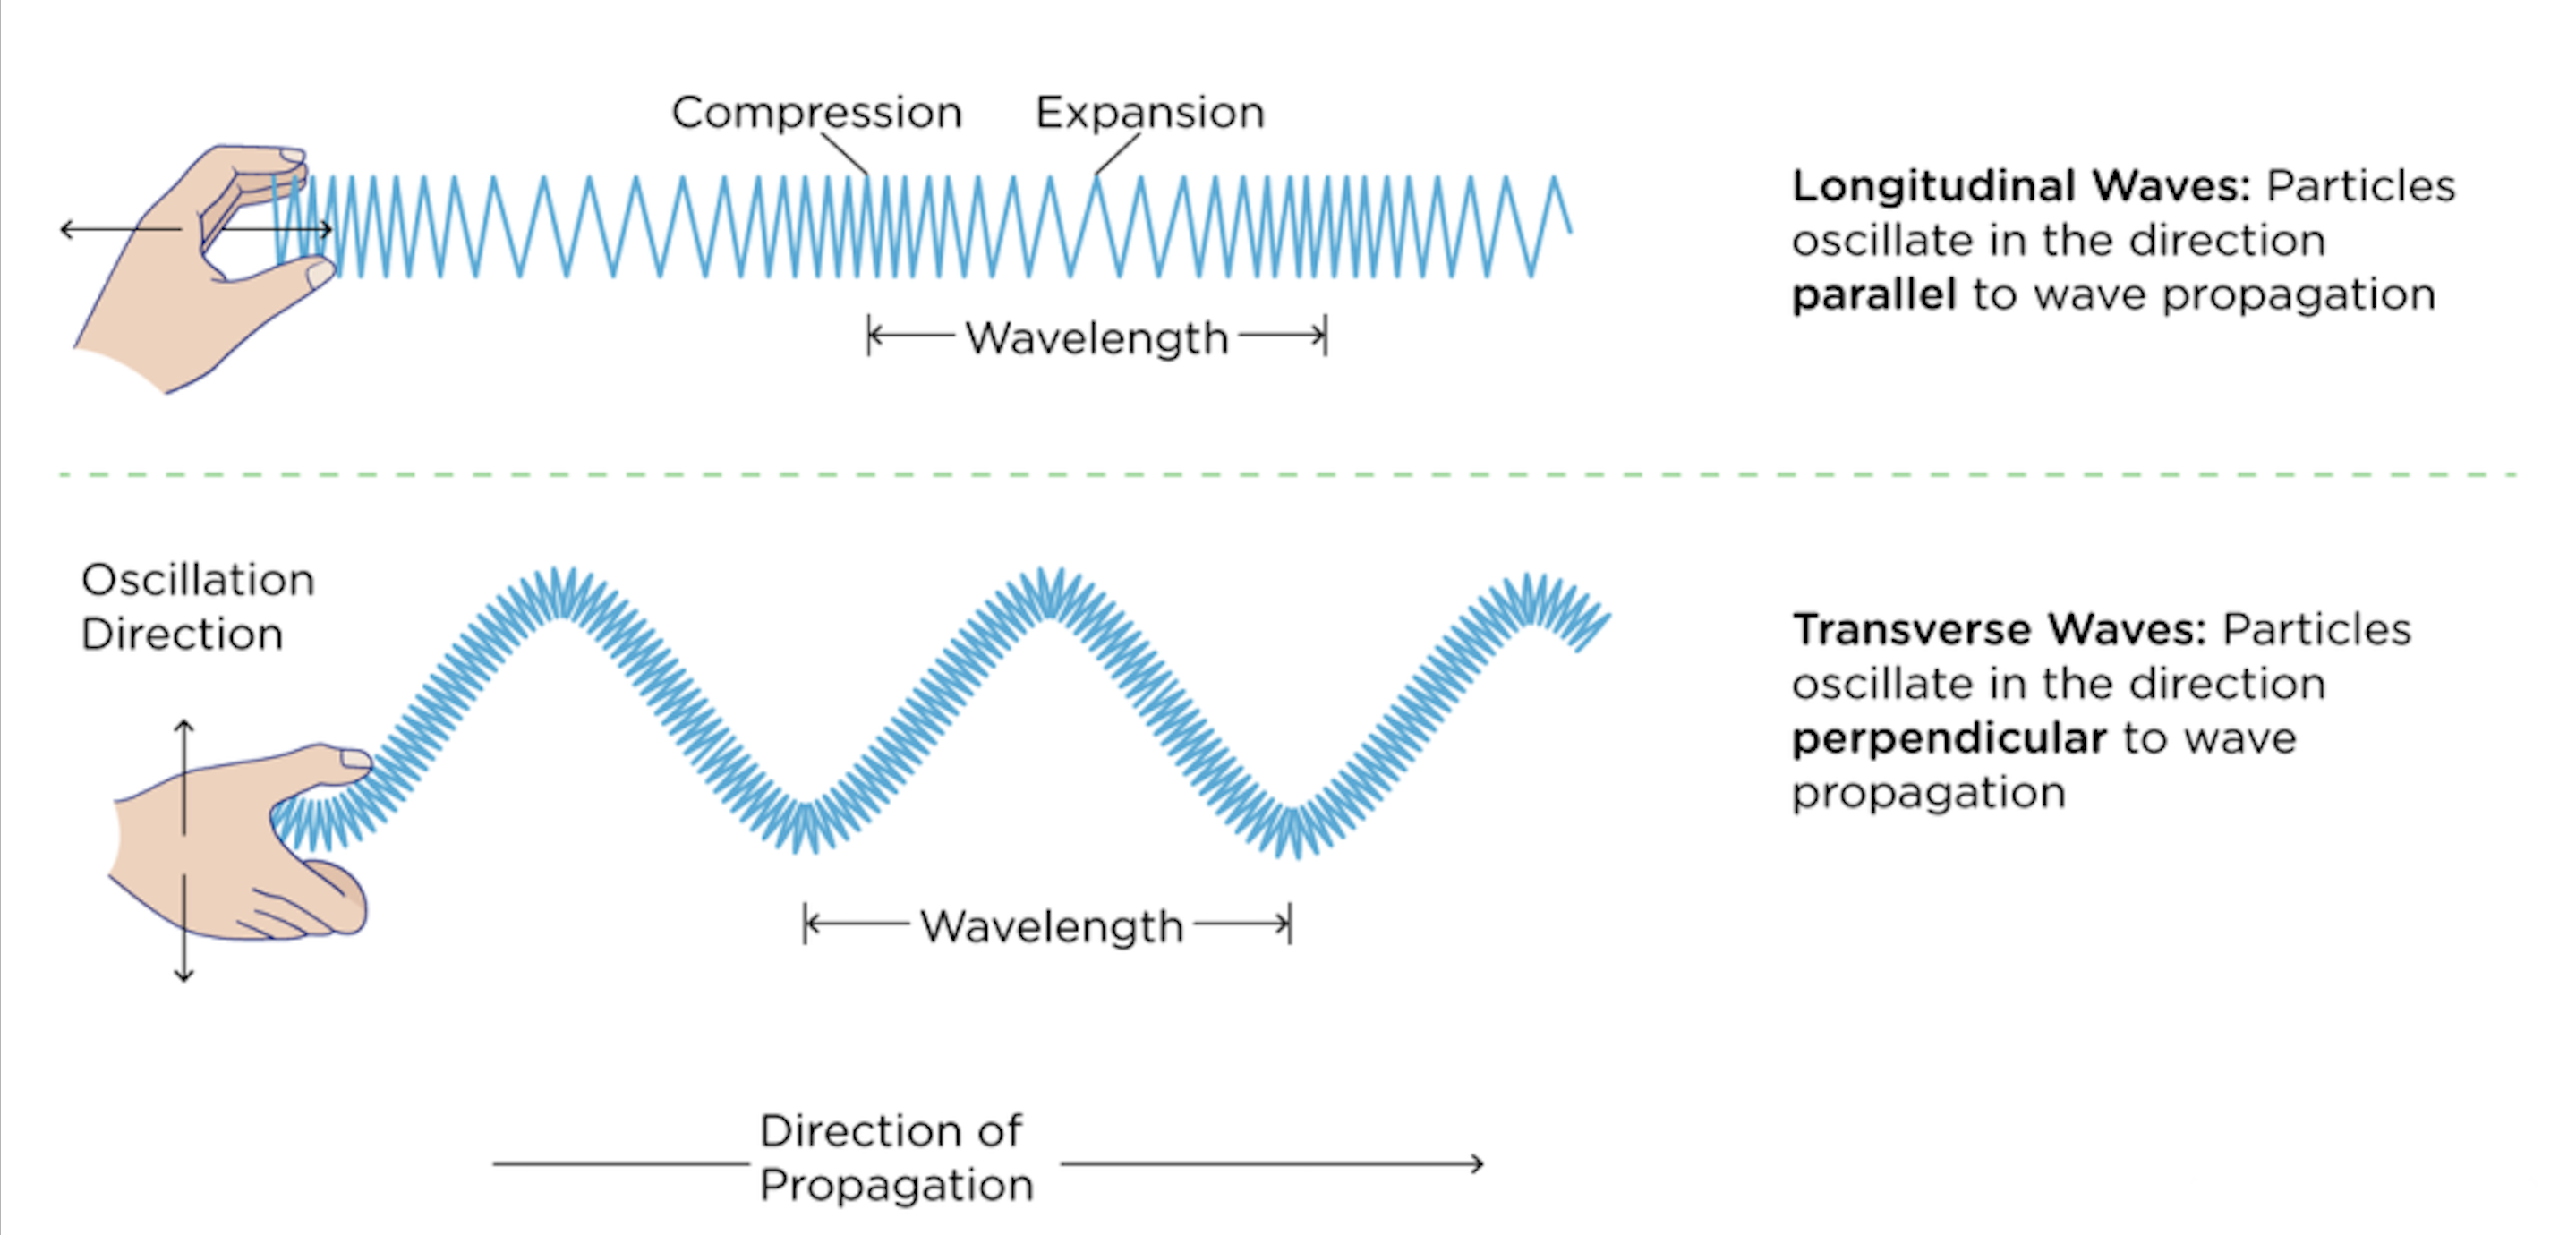
\includegraphics[height = 7 cm ]{Bilder/Wellen longitudinal, transversal .png}
    
    \caption{\footnotesize  Longitudinalwave (top) and transverse  wave (bottom)}
    \label{img: wave types}

    %Quelle: https://www.researchgate.net/figure/llustration-of-a-transverse-wave-and-a-longitudinal-wave_fig6_334074508%
\end{center}
\end{figure}

\textbf{Sound waves are longitudinal waves.} When a loudspeaker or a vibrating string moves back and forth, it pushes the surrounding air particles together and pulls them apart alternately. These pressure variations propagate through the air and eventually reach our ears, where they are perceived as sound.


\subsubsection{Mechanical Waves in Acoustics}

Now that we understand what mechanical waves are, we can take a closer look at how they appear in acoustics.

\paragraph{Sound as a Pressure Wave}
Sound is a longitudinal mechanical wave that propagates through an elastic medium such as air, water, or solid materials. The vibrating source -- for example a guitar string or a loudspeaker membrane -- causes the surrounding air molecules to oscillate back and forth. This creates alternating regions of high pressure (compressions) and low pressure (rarefactions) that travel through the air as a wave.

\begin{figure}
    \centering
    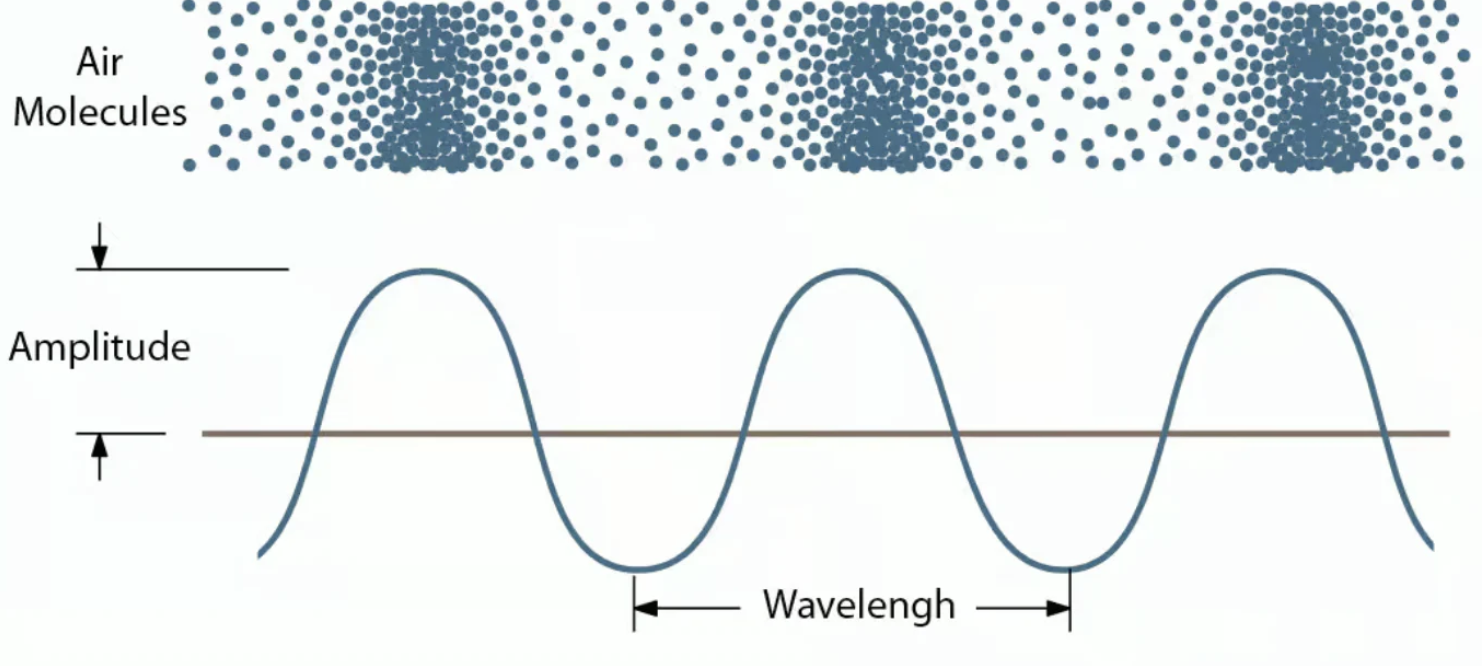
\includegraphics[width=0.5\linewidth]{Bilder/Schallwelle.png}
    \caption{propagation of a sound wave by moving air particles}
    %Quelle : https://scienceready.com.au/pages/properties-of-longitudinal-waves?srsltid=AfmBOooII3UfO-C_-FxYRDm-lTvWtuxHEt6kLbHXJp3DsEo41Hkc5vyy%
    \label{fig:placeholder}
\end{figure}

\paragraph{Speed of Sound}
Sound travels through air at approximately
\begin{equation}
    c_{\text{sound}} \approx 343 \, \frac{\text{m}}{\text{s}}
\end{equation}
at room temperature. This is much slower than the speed of light ($c_{\text{light}} \approx 3 \times 10^8 \, \frac{\text{m}}{\text{s}}$). You experience this difference every time there is a thunderstorm: you see the lightning almost instantly, but the sound of the thunder arrives several seconds later.

\paragraph{Frequency and Pitch}
The frequency of a sound wave determines the pitch you perceive:
\begin{itemize}
    \item \textbf{High frequency} $\Rightarrow$ high pitch 
    \item \textbf{Low frequency} $\Rightarrow$ low pitch 
\end{itemize}
The human ear can perceive sounds in the frequency range of approximately
\begin{equation}
    20 \, \text{Hz} \leq f \leq 20{,}000 \, \text{Hz}
\end{equation}
Sounds below 20\,Hz are called \textbf{infrasound} -- these are too low for humans to hear, but some animals such as elephants use them to communicate over long distances. Sounds above 20{,}000\,Hz are called \textbf{ultrasound} -- bats and dogs can perceive these frequencies.

\begin{table}[h]
\centering
\begin{tabular}{|l|c|}
\hline
\textbf{Sound} & \textbf{Frequency} \\
\hline
Infrasound (inaudible) & $< 20\,\text{Hz}$ \\
Human hearing range   & $20\,\text{Hz} - 20{,}000\,\text{Hz}$ \\
Middle A (concert pitch) & $440\,\text{Hz}$ \\
Ultrasound (inaudible) & $> 20{,}000\,\text{Hz}$ \\
\hline
\end{tabular}
\caption{Frequency ranges relevant to acoustics}
\label{tab:frequencies}
\end{table}
The amplitude of the oscillation determines the volume level of the sound. The greater the amplitude, the louder the sound becomes.

\subsubsection{Superposition of Waves}

\paragraph{Principle of Superposition:}
When multiple waves meet at a point, they overlap. This means that the displacements of the individual waves simply add up at every point, resulting in a new combined wave. The wave that results from this superposition is called the \textbf{resulting wave}.

A helpful analogy: imagine two people throwing stones into a calm lake at the same time. Where the ripples from both stones meet, they overlap -- sometimes creating bigger waves, sometimes cancelling each other out.

If waves with the same frequency meet, they can either reinforce or weaken each other depending on their \textbf{phase relationship} -- that is, how their peaks and troughs line up:

\begin{itemize}
    \item \textbf{Constructive interference}: the peaks of both waves align. The amplitudes add up, and the resulting wave is larger than either individual wave.
    \item \textbf{Destructive interference}: the peak of one wave aligns with the trough of the other. The amplitudes cancel out, and the resulting wave has a smaller amplitude -- in the ideal case, the waves cancel completely.
\end{itemize}

Both phenomena are shown in Figure \ref{img: Interferenz}.

\begin{figure}[!ht]
\begin{center}
    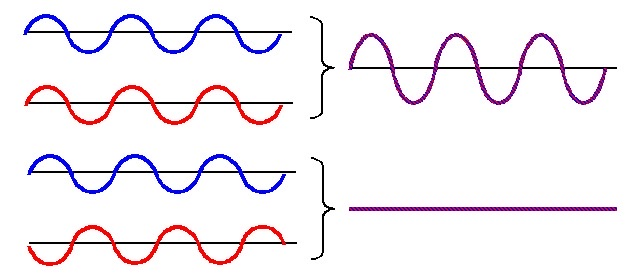
\includegraphics[height=4cm]{Bilder/Interferenz.jpeg}
    \caption{\footnotesize interference phenomena}
    \label{img: Interferenz}
\end{center}
\end{figure}

\textit{Real-world example:} Noise-cancelling headphones use destructive interference. A microphone picks up the surrounding noise, and the headphones produce a wave with exactly the opposite phase -- the two waves cancel each other out, and you hear silence.

\paragraph{Standing Waves:}

A particularly important special case of superposition occurs when two waves with the \textbf{same wavelength and frequency travel in opposite directions} and overlap. The result is a so-called \textbf{standing wave}.

Unlike a normal (travelling) wave, a standing wave does not appear to move through space. Instead, certain points remain permanently at rest, while others oscillate with maximum amplitude. The following terms are used:

\begin{itemize}
    \item \textbf{Nodes (N)}: points that remain permanently at rest
    \item \textbf{Antinodes (A)}: points that oscillate with maximum amplitude
\end{itemize}

Nodes and antinodes alternate regularly, always separated by a distance of:
\begin{equation}
    \Delta x = \frac{\lambda}{4}
\end{equation}

Figure \ref{img: stehende Welle} shows a standing wave at different moments in time. Notice how the wave pattern does not travel -- it simply oscillates up and down in place.

\begin{figure}[!ht]
    \centering
    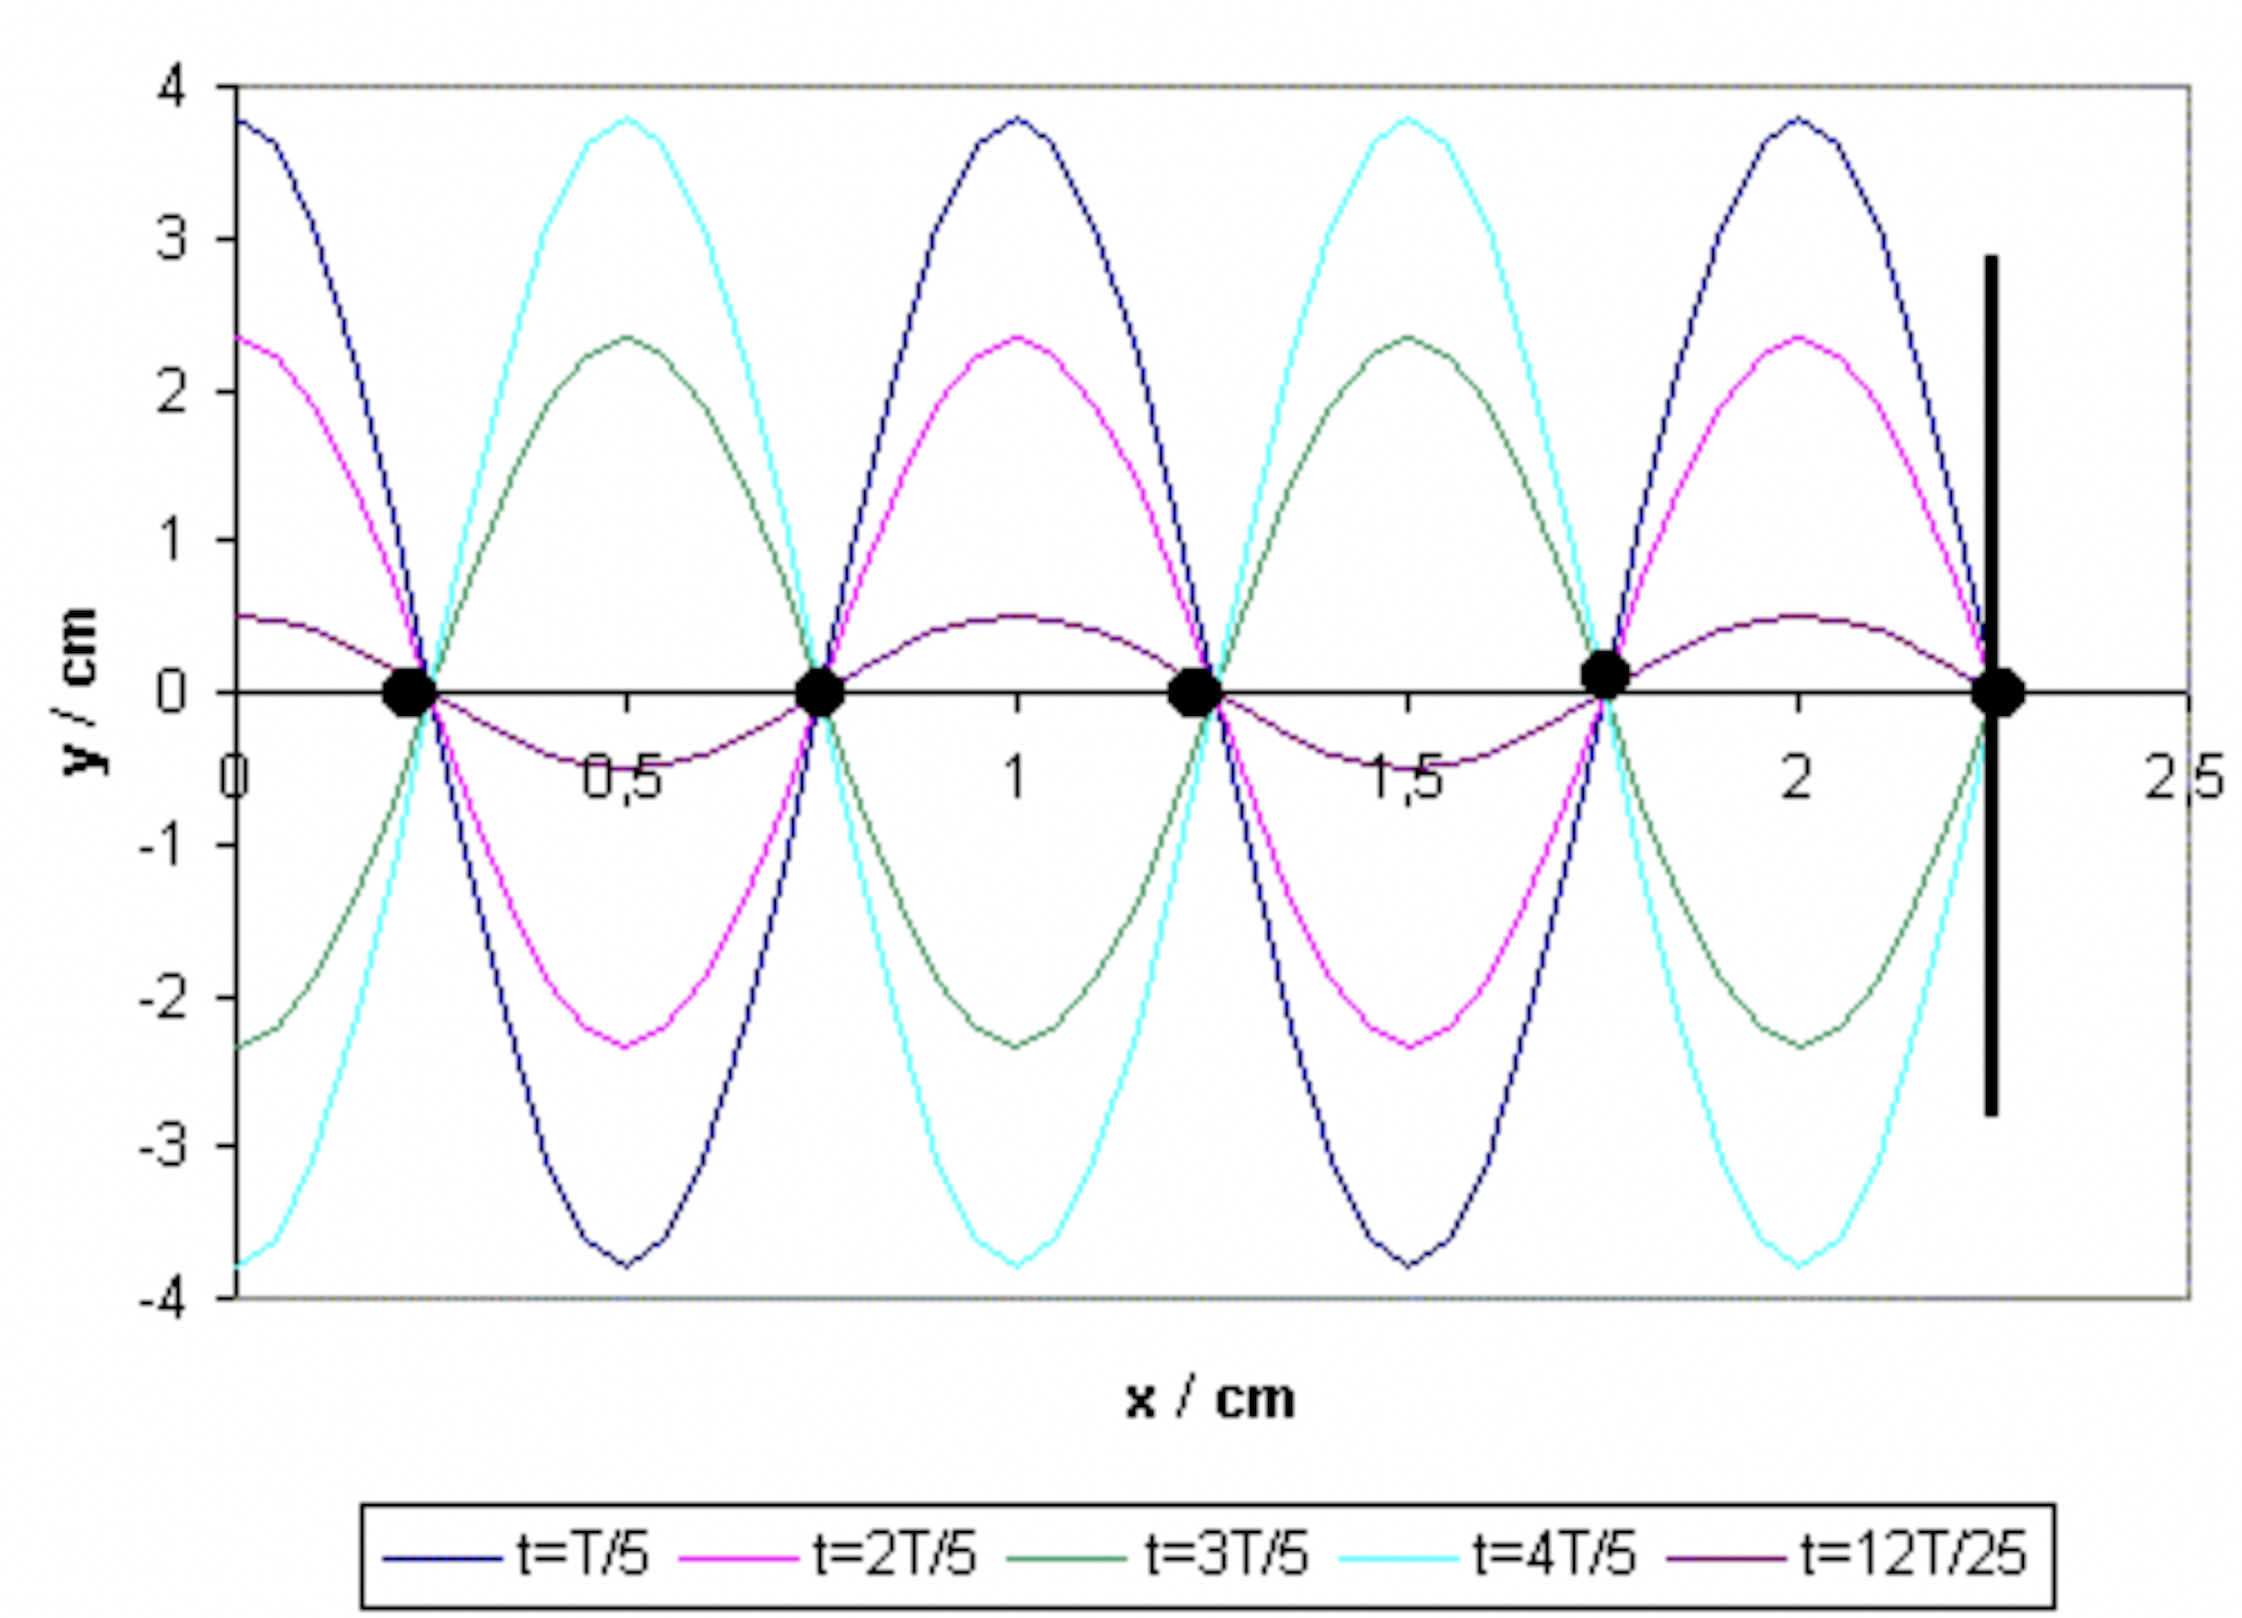
\includegraphics[height=6cm]{Bilder/stehende Welle.png}
    \caption{standing wave at different times}
    \label{img: stehende Welle}
\end{figure}

\paragraph{Harmonics -- At Which Frequencies Do Standing Waves Occur?}
Standing waves can only form at specific frequencies. These depend on the \textbf{length of the medium} (e.g. a string or a air column) and on the \textbf{boundary conditions} -- that is, what happens at the ends of the medium. We distinguish three important cases:

\subparagraph{Case 1: One Fixed End, One Free End}

A \textbf{fixed end} is always a node (the medium cannot move there). A \textbf{free end} is always an antinode (the medium can oscillate freely).

\textit{Example:} A rope attached to a wall at one end, which you shake at the other end, sound waves in a test tube

Standing waves can form when the length $l$ of the medium satisfies:
\begin{equation}
    l = \frac{2n+1}{4} \cdot \lambda = \frac{(2n+1) \cdot c}{4f} \qquad n \in \mathbb{N}_0
\end{equation}

The table below shows the first few allowed cases:

\begin{table}[h]
\centering
\begin{tabular}{|c|c|c|l|}
\hline
$n$ & Condition & Sketch & Description \\
\hline
0 & $l = \dfrac{\lambda}{4}$ & N---A & fundamental mode (1st harmonic) \\[6pt]
1 & $l = \dfrac{3\lambda}{4}$ & N-A-N-A & 2nd harmonic \\[6pt]
2 & $l = \dfrac{5\lambda}{4}$ & N-A-N-A-N-A & 3rd harmonic \\[6pt]
\hline
\end{tabular}
\caption{Standing waves with one fixed and one free end}
\label{tab:harmonics_one_fixed}
\end{table}
\begin{figure}
    \centering
    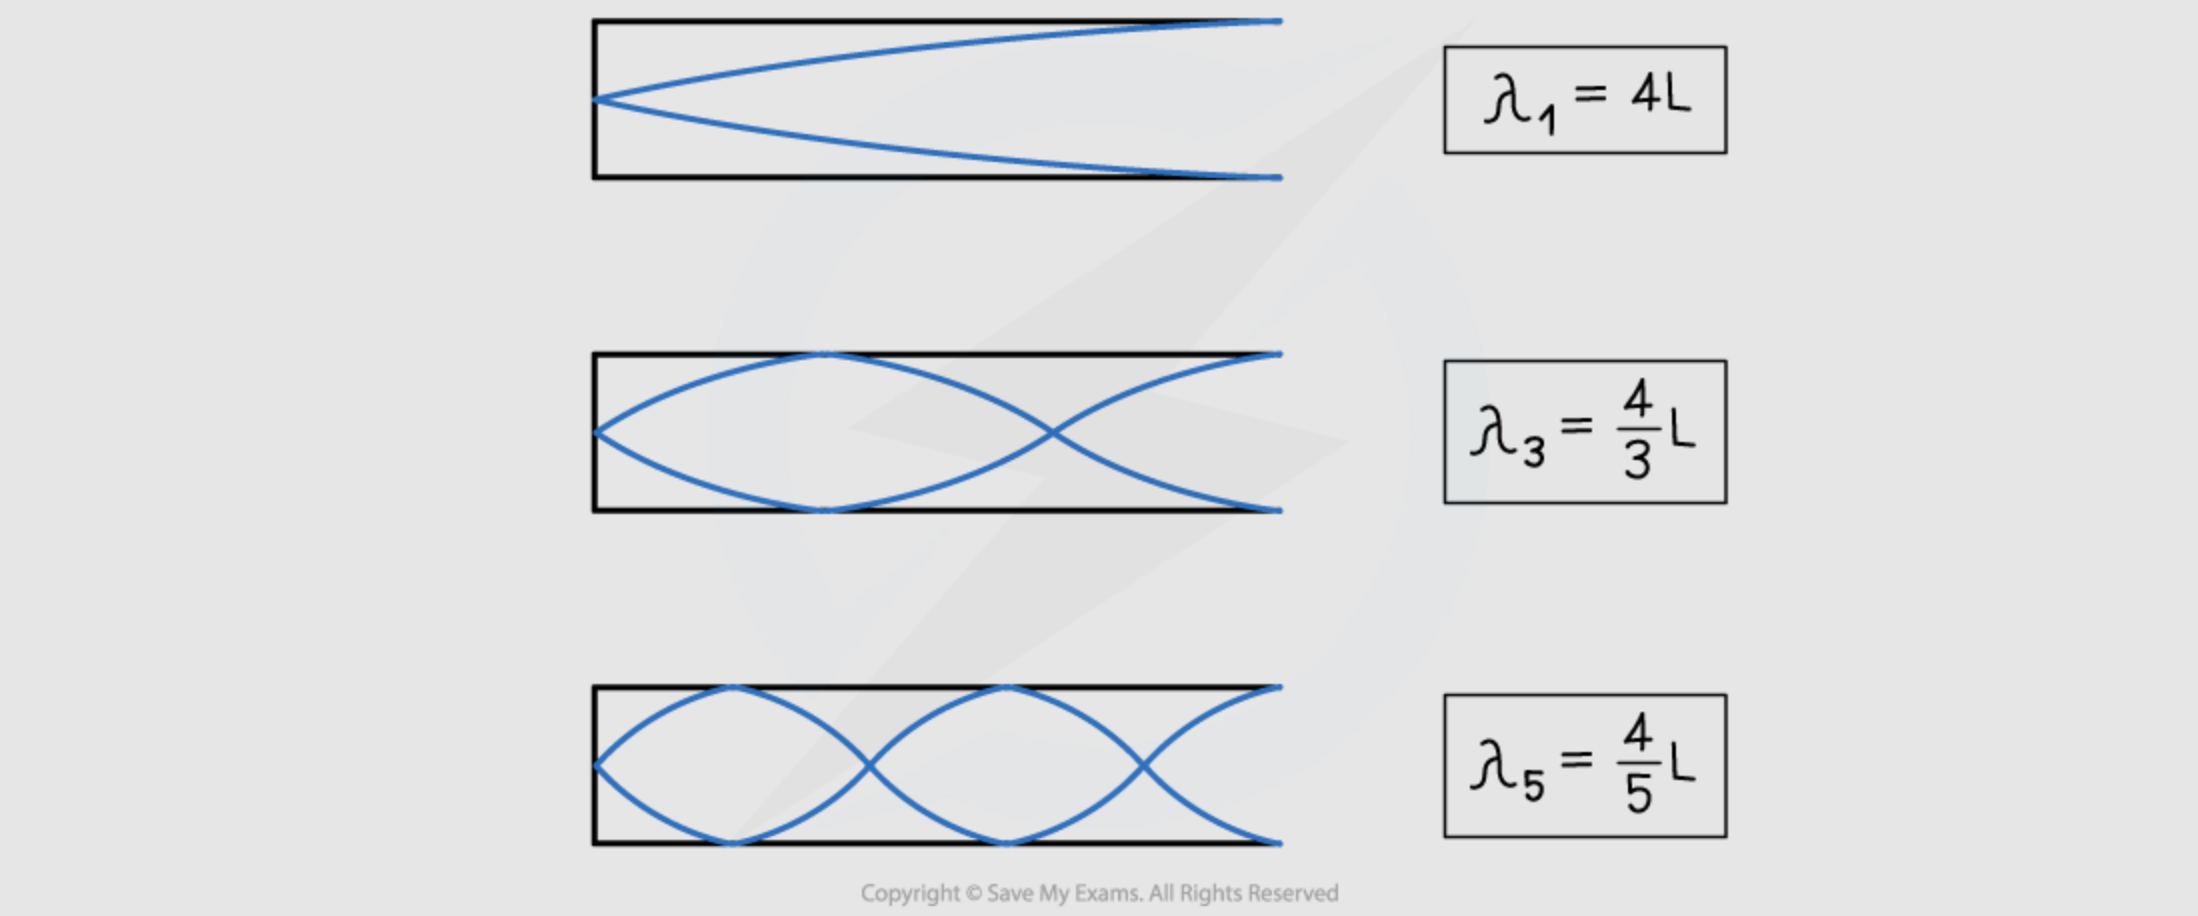
\includegraphics[width=0.5\linewidth]{Bilder/unterschiedliche Enden harmoics.png}
    \caption{Harmonic waves in a medium with a fixed end and a free end }
    \label{fig:different ends - harmonics }
    %Quelle: https://www.savemyexams.com/dp/physics/ib/23/sl/revision-notes/wave-behaviour/standing-waves-and-resonance/harmonics-in-strings-and-pipes/%
\end{figure}

\textit{Musical application:} A simple and convincing experiment illustrates this case: 
if you blow across the opening of a test tube, you produce a sound. 
The closed bottom of the test tube is a \textbf{fixed end} and therefore always a \textbf{node}, 
while the open top is a \textbf{free end} and therefore always an \textbf{antinode}. 
The simplest standing wave that can form under these conditions has exactly one node (at the bottom) 
and one antinode (at the top) -- this corresponds to $n=0$, i.e.:
\begin{equation}
    l = \frac{\lambda}{4}
\end{equation}
The length of the test tube equals exactly one quarter of the wavelength. 
This is the \textbf{fundamental mode}: the lowest frequency at which a standing wave can form, 
and therefore the pitch you hear when blowing across the tube. 
The longer the test tube, the longer the wavelength -- and the lower the pitch. 
This is why filling the test tube with water (and thus shortening the air column) produces a higher tone.
Only odd harmonics are present in this system, giving it a characteristic hollow sound.

\subparagraph{Case 2: Two Fixed Ends} 

Both ends are fixed and thus nodes. \\ 
\textit{Example:} A \textbf{string fixed at both ends}, such as a guitar or violin string 

In this case, standing waves form when the following condition is fulfilled:
\begin{equation}
    l = \frac{n}{2} \cdot \lambda = \frac{n \cdot c}{2f} \qquad n \in \mathbb{N}
\end{equation}

\begin{table}[h]
\centering
\begin{tabular}{|c|c|c|l|}
\hline
$n$ & Condition & Sketch & Description \\
\hline
1 & $l = \dfrac{\lambda}{2}$ & N---A---N & fundamental mode (1st harmonic) \\[6pt]
2 & $l = \lambda$ & N-A-N-A-N & 2nd harmonic (1st overtone) \\[6pt]
3 & $l = \dfrac{3\lambda}{2}$ & N-A-N-A-N-A-N & 3rd harmonic (2nd overtone) \\[6pt]
\hline
\end{tabular}
\caption{Standing waves with two fixed ends}
\label{tab:harmonics_two_fixed}
\end{table}
\begin{figure}
    \centering
    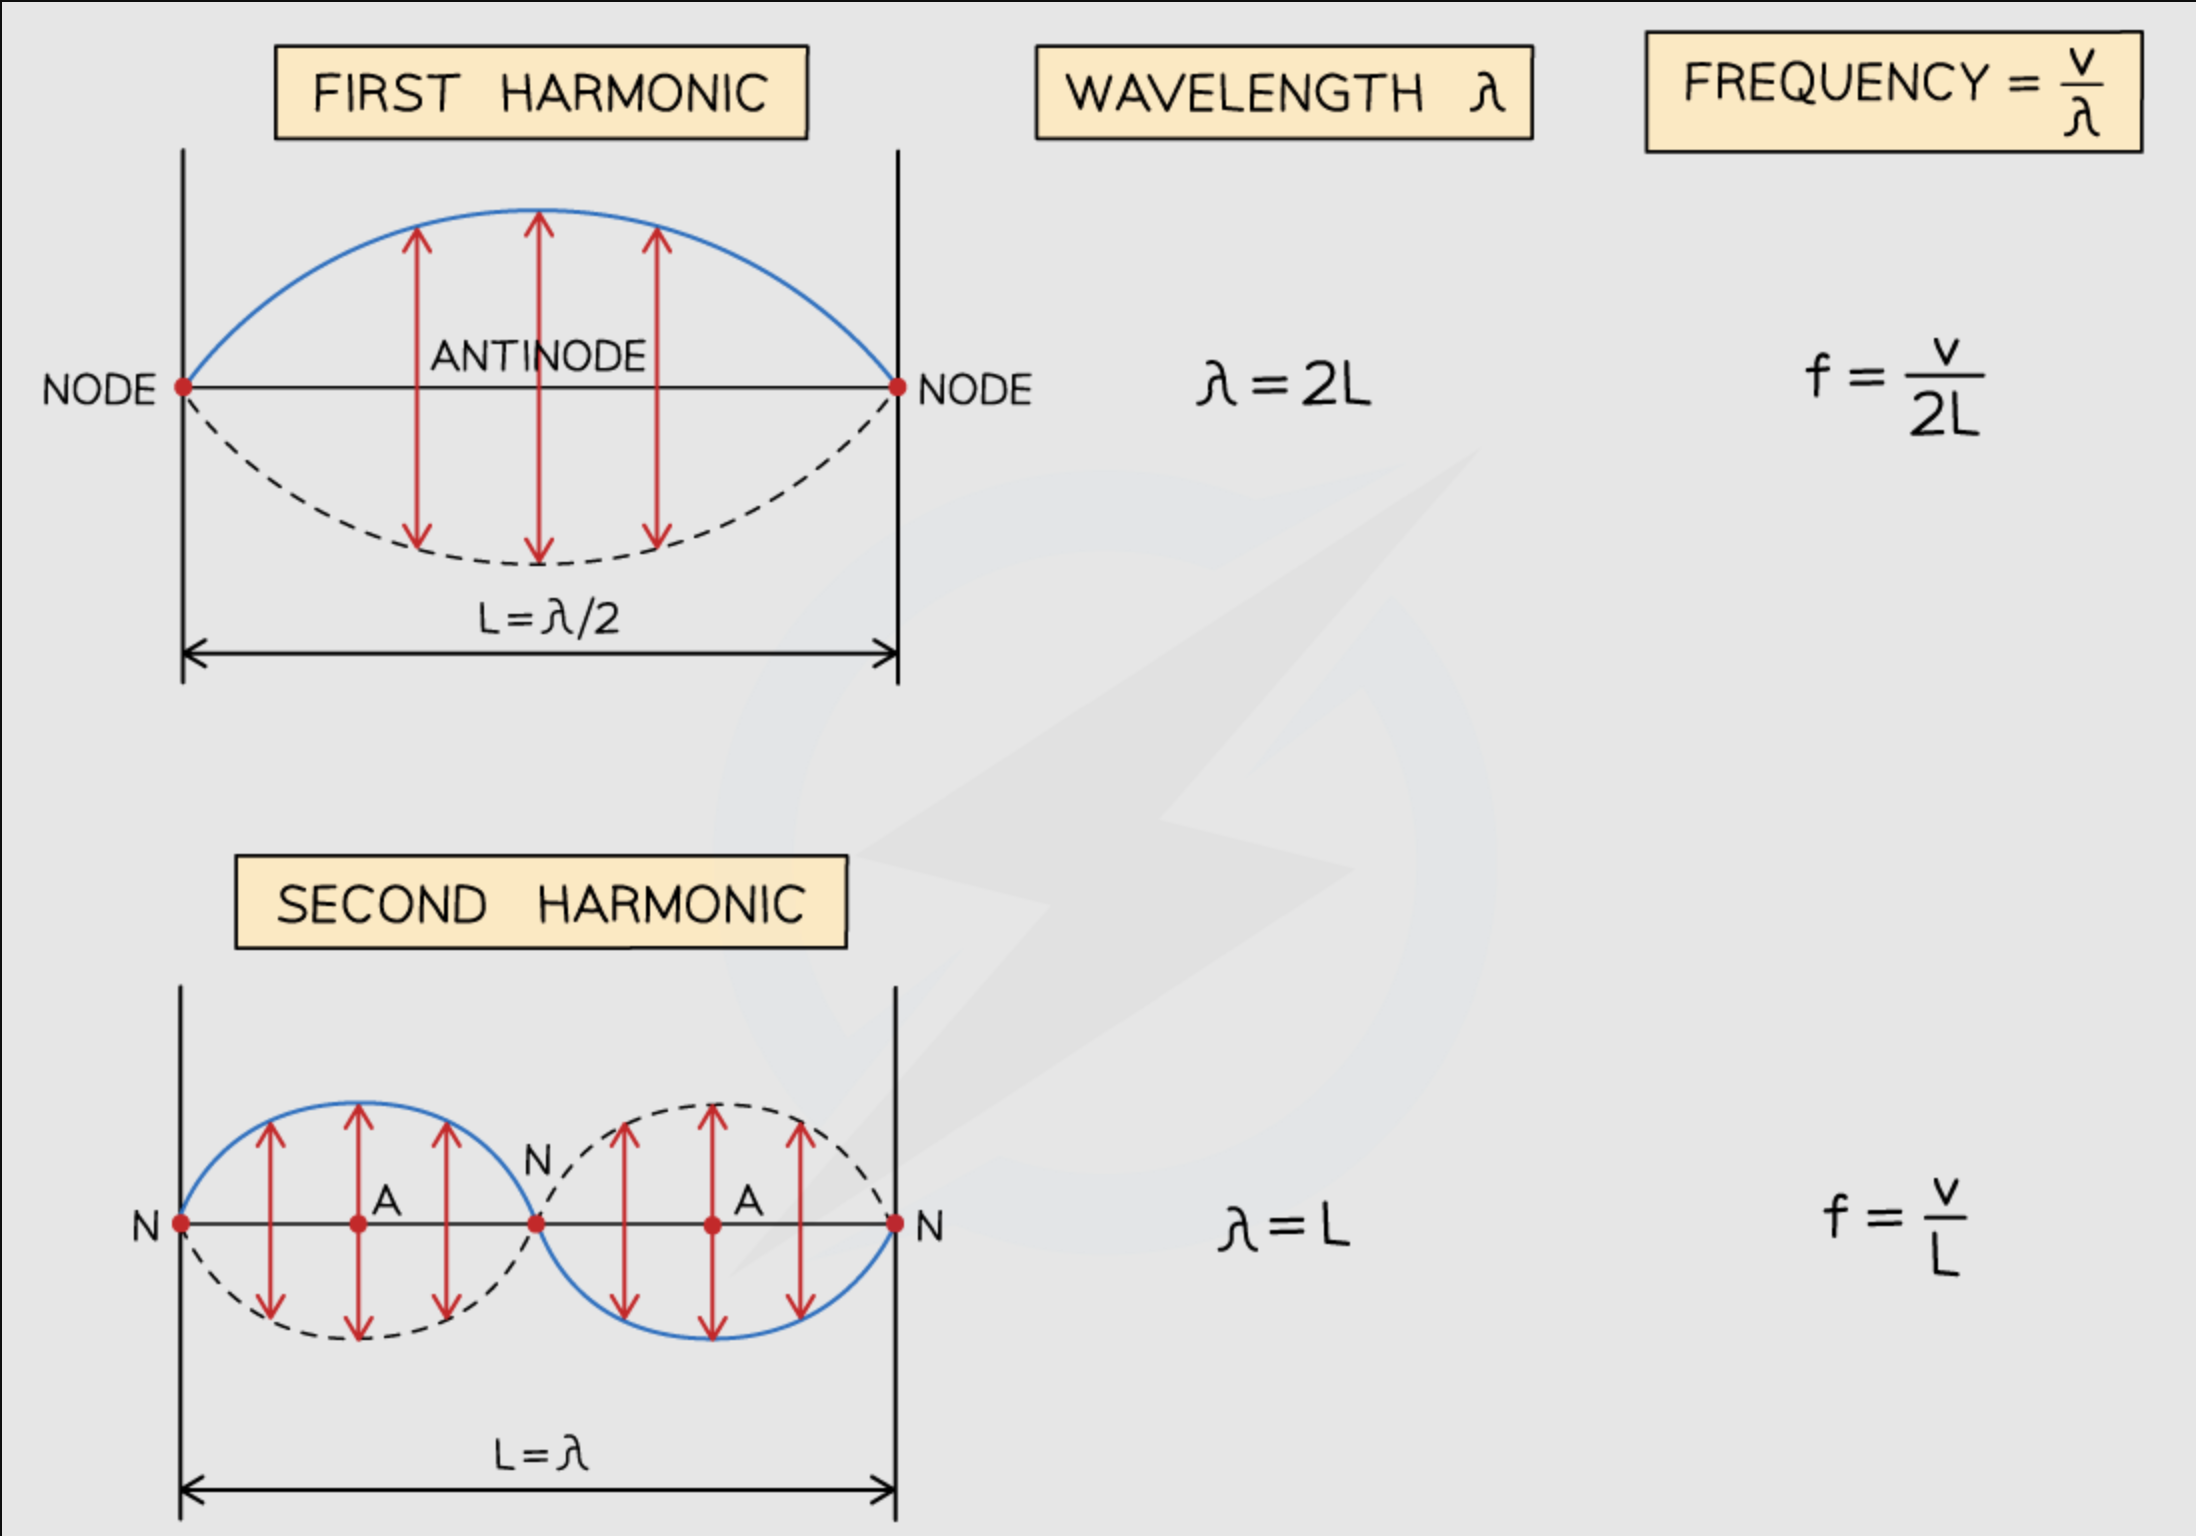
\includegraphics[width=0.5\linewidth]{Bilder/feste Enen harmonics.png}
    \caption{Harmonic waves in a medium with fixed ends }
    \label{fig:different ends - harmonics }
\end{figure}
\subparagraph{Case 3: Two Free Ends}

Both ends are free and thus antinodes. 
\textit{Example:} wind instruments open at both ends such as an open organ pipe 

The condition is the same as for two fixed ends:
\begin{equation}
    l = \frac{n}{2} \cdot \lambda = \frac{n \cdot c}{2f} \qquad n \in \mathbb{N}
\end{equation}
\begin{figure}
    \centering
    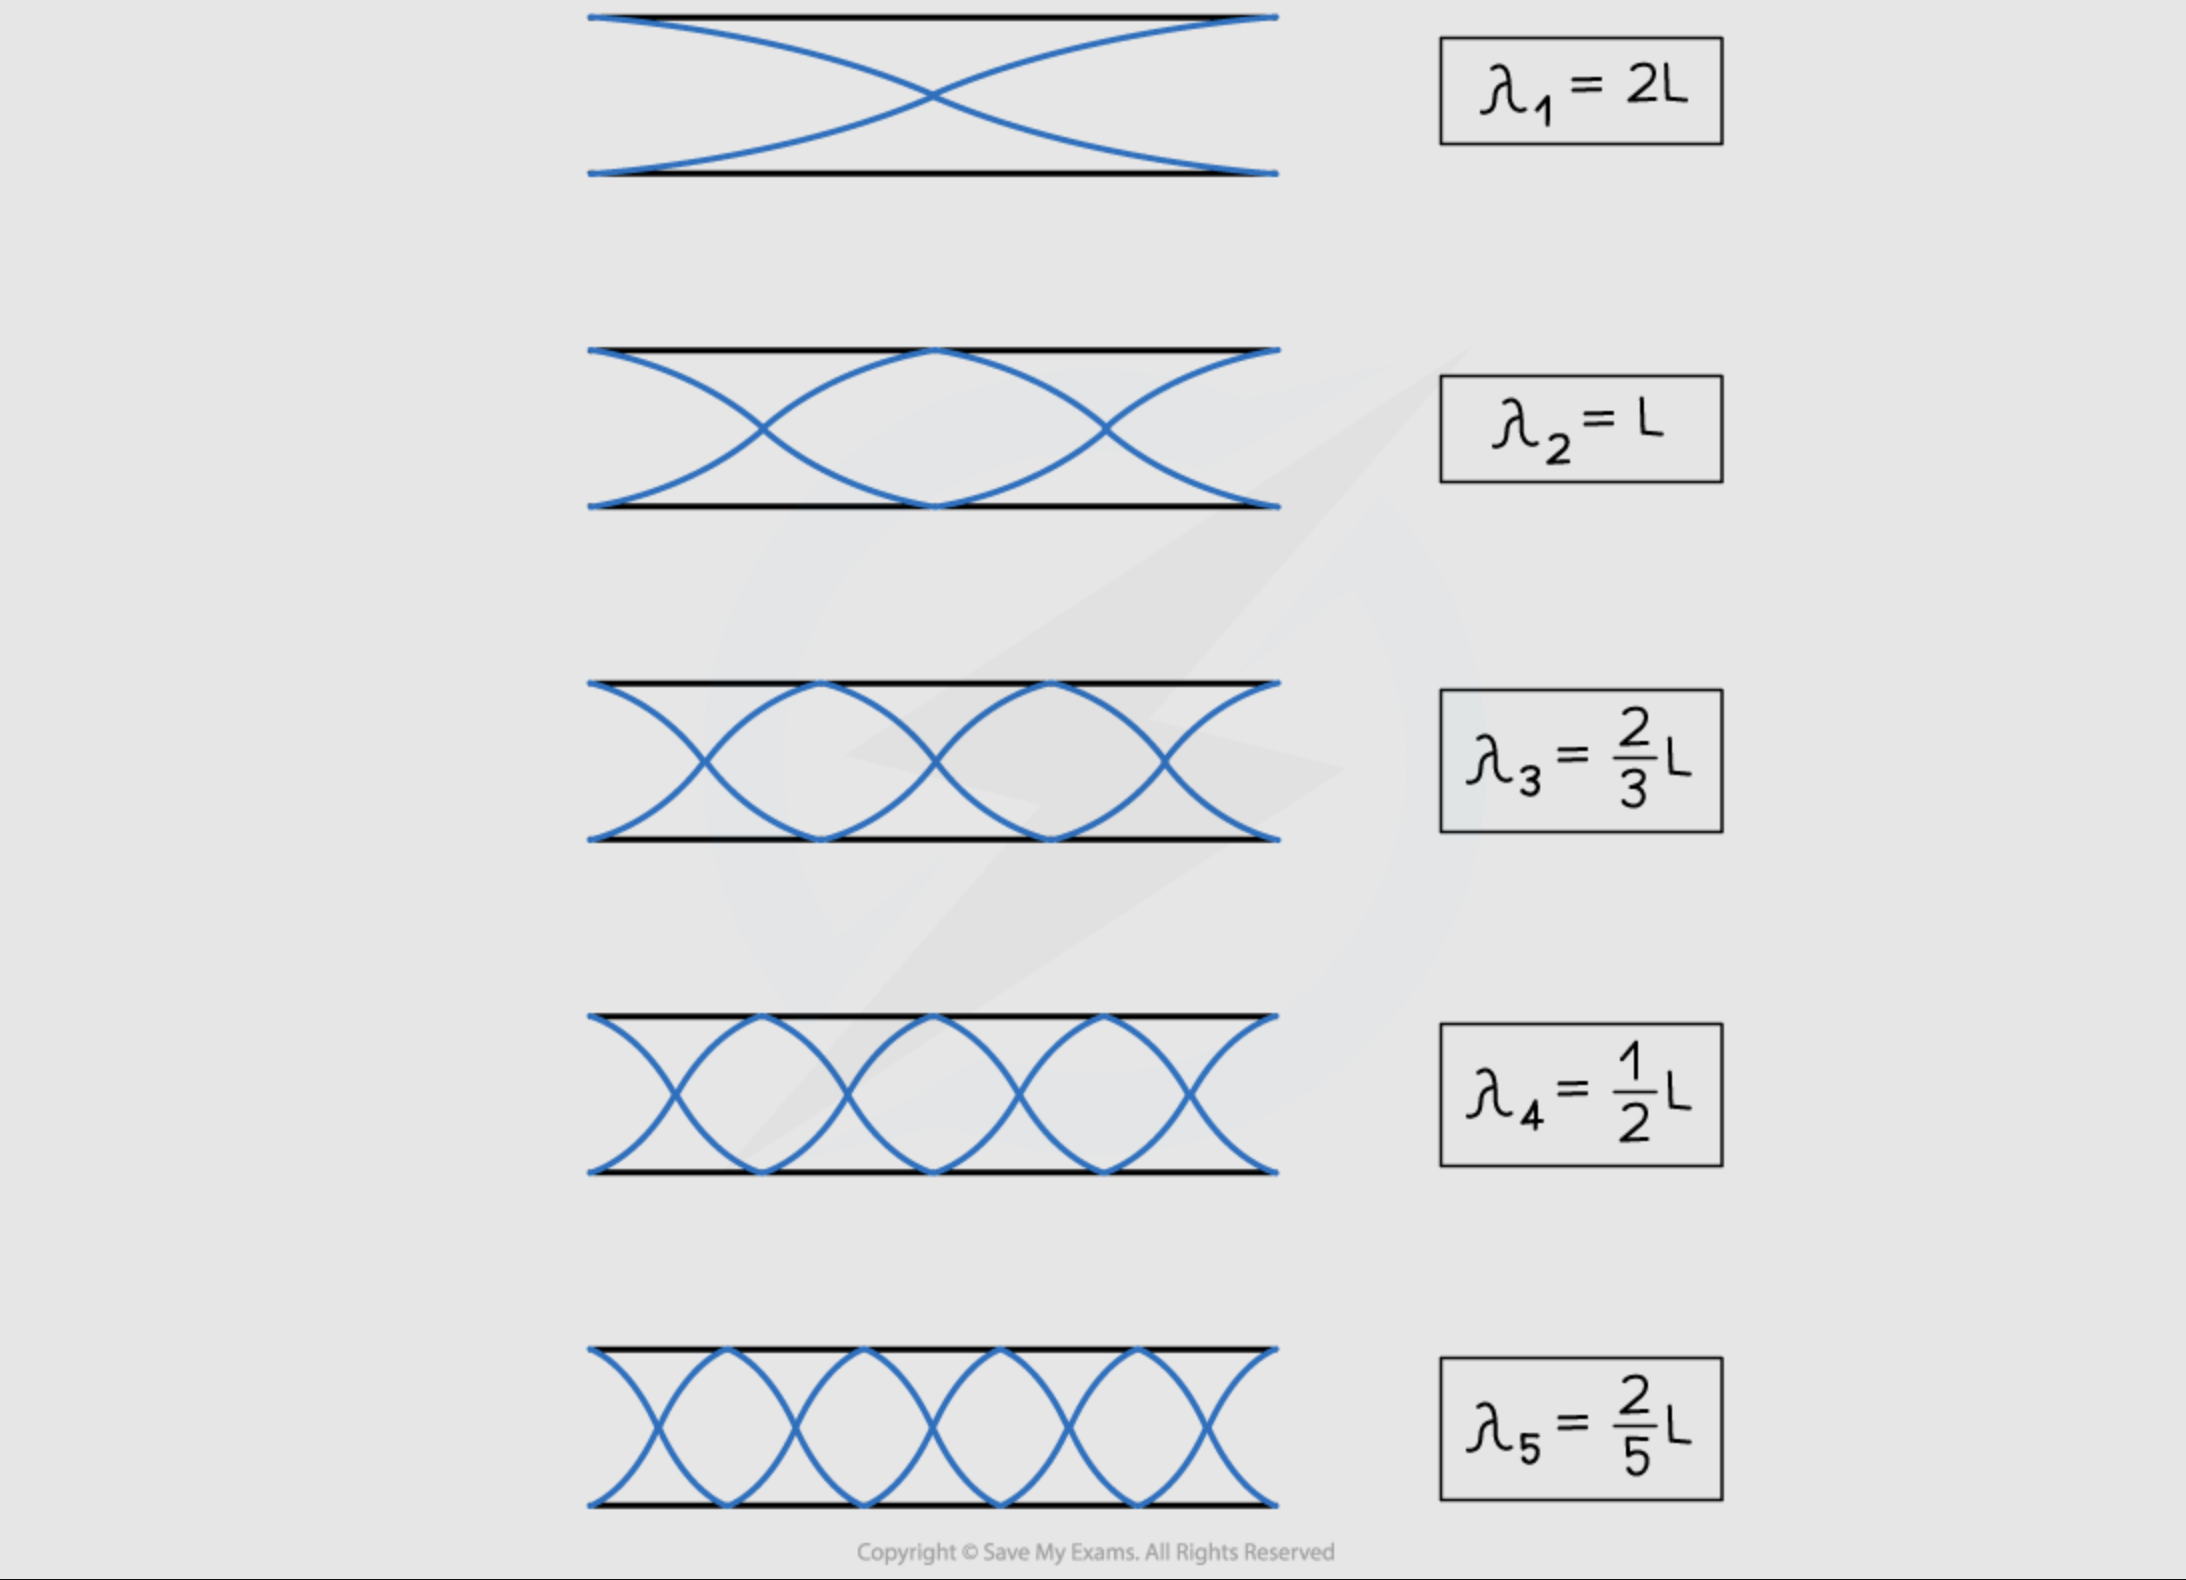
\includegraphics[width=0.5\linewidth]{Bilder/lose Enden harmonics.png}
    \caption{Harmonic waves in a medium with free ends}
    \label{fig:free ends harmonics}
\end{figure}

Although the condition for the wavelength looks identical to Case 2
the standing wave pattern on the medium looks different. The key difference lies in the 
\textbf{boundary conditions} -- that is, what happens at the ends. Think of it this way: the mathematical condition $l = \frac{n}{2}\lambda$ tells you 
\textit{how many half-wavelengths fit into the medium} -- but the boundary conditions 
tell you \textit{where exactly the wave starts and ends}. 

\paragraph{Summary: Boundary Conditions and Their Effects}

\begin{comment}


\begin{figure}
    \centering
    \includegraphics[width=0.5\linewidth]{}
    \caption{Caption}
    \label{fig:placeholder}
\end{figure}
\end{comment}

\begin{table}[h]
\centering
\begin{tabular}{|l|c|c|l|}
\hline
\textbf{Boundary condition} & \textbf{Condition} & \textbf{Harmonics present} & \textbf{Example} \\
\hline
One fixed, one free end & $l = \frac{(2n+1)}{4}\lambda$ & odd only (1st, 3rd, 5th \ldots) & closed wind instrument \\
Two fixed ends          & $l = \frac{n}{2}\lambda$      & all (1st, 2nd, 3rd \ldots)      & string instrument \\
Two free ends           & $l = \frac{n}{2}\lambda$      & all (1st, 2nd, 3rd \ldots)      & open organ pipe \\
\hline
\end{tabular}
\caption{Overview of boundary conditions for standing waves}
\label{tab:boundary_conditions}
\end{table}
The \textbf{1st harmonic} (or \textbf{fundamental}) is always the lowest 
frequency at which a standing wave can form in a given medium -- it has the fewest possible 
nodes and antinodes. The \textbf{2nd harmonic} has exactly twice the frequency of the 
fundamental, the \textbf{3rd harmonic} three times, and so on. Each higher harmonic fits 
one additional half-wavelength into the medium. When you play a musical instrument, 
you typically hear the fundamental as the \textbf{pitch}, while the mix of higher harmonics 
shapes the \textbf{timbre} - we will discuss this in  detail later on. 
